\documentclass[tikz]{standalone}
\usepackage{amsmath,amssymb}
\usetikzlibrary{arrows.meta}

% Classes of morphisms
\newcommand{\all}{\mathsf{all}}
\newcommand{\inj}{\mathsf{inj}}
\newcommand{\surj}{\mathsf{surj}}
\newcommand{\bij}{\mathsf{bij}}
\newcommand{\init}{\mathsf{init}}
\newcommand{\pb}{\mathsf{pb}}
\newcommand{\homog}{\mathsf{homog}}
\DeclareMathOperator{\id}{id}
\renewcommand\emptyset\varnothing
\begin{document}
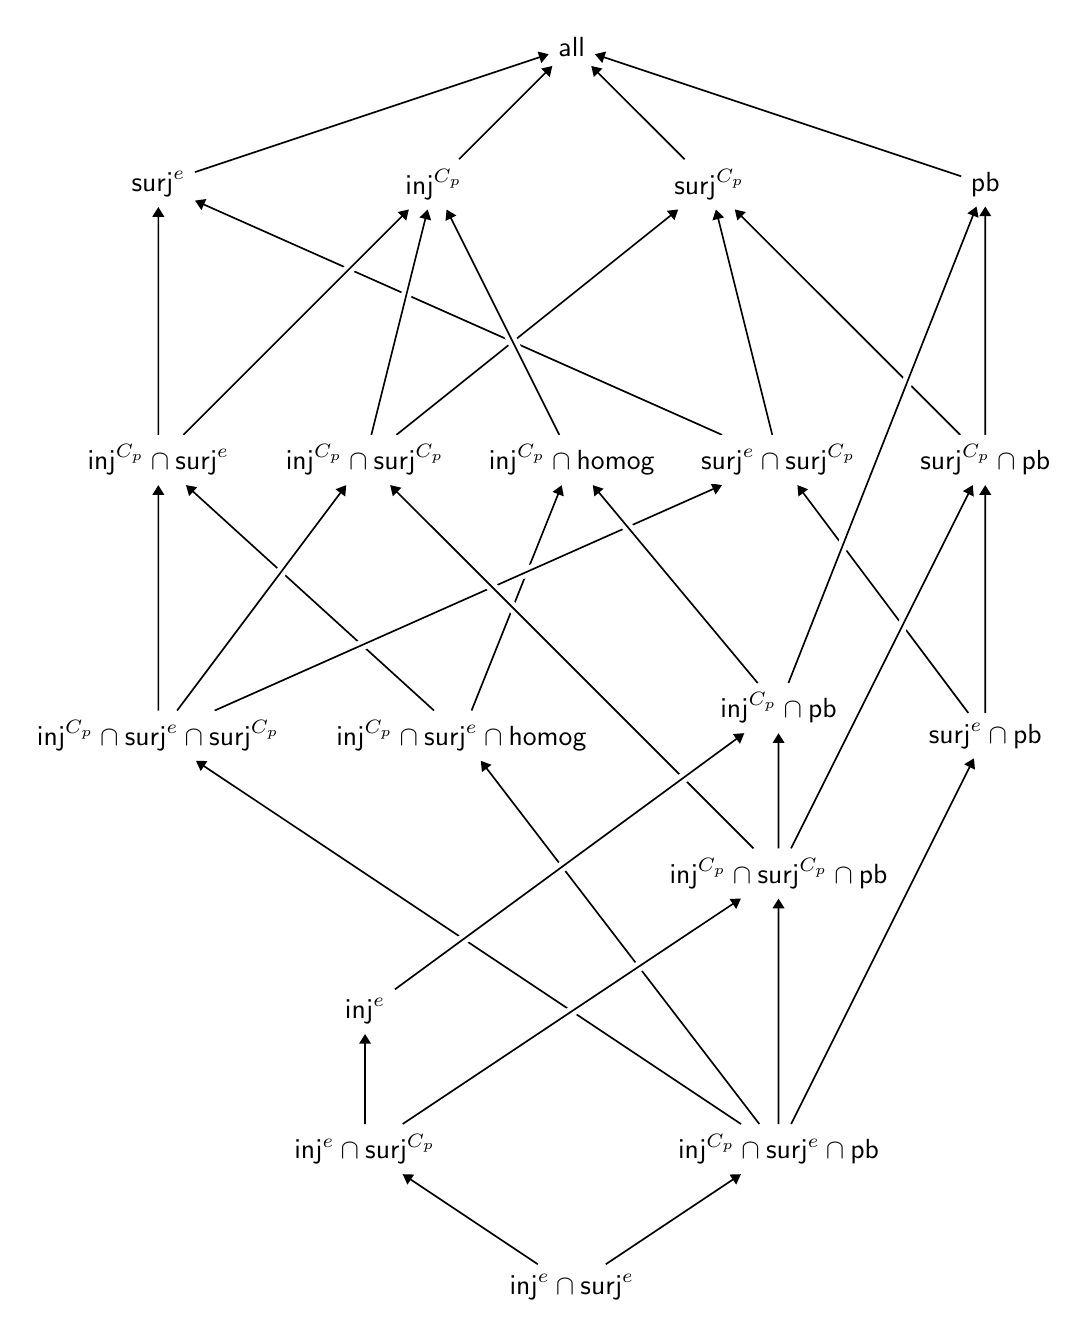
\begin{tikzpicture}[scale=3.5]
	\node (v0) at (0, 2) {$ \all $};
	\node (v1) at (-0.5, 1.5) {$ \inj^{C_p} $};
	\node (v2) at (-1.5, 1.5) {$ \surj^e $};
	\node (v3) at (0.5, 1.5) {$ \surj^{C_p} $};
	\node (v4) at (-1.5, 0.5) {$ \inj^{C_p} \cap \surj^e $};
	\node (v5) at (-0.75, 0.5) {$ \inj^{C_p} \cap \surj^{C_p} $};
	\node (v6) at (0, 0.5) {$ \inj^{C_p} \cap \homog $};
	\node (v7) at (0.75, 0.5) {$ \surj^e \cap \surj^{C_p} $};
	\node (v8) at (1.5, 1.5) {$ \pb $};
	\node (v9) at (-1.5, -0.5) {$ \inj^{C_p} \cap \surj^e \cap \surj^{C_p} $};
	\node (v10) at (-0.4, -0.5) {$ \inj^{C_p} \cap \surj^e \cap \homog $};
	\node (v11) at (0.75, -0.4) {$ \inj^{C_p} \cap \pb $};
	\node (v12) at (1.5, 0.5) {$ \surj^{C_p} \cap \pb $};
	\node (v13) at (-0.75, -1.5) {$ \inj^e $};
	\node (v14) at (0.75, -1) {$ \inj^{C_p} \cap \surj^{C_p} \cap \pb $};
	\node (v15) at (1.5, -0.5) {$ \surj^e \cap \pb $};
	\node (v16) at (-0.75, -2) {$ \inj^e \cap \surj^{C_p} $};
	\node (v17) at (0.75, -2) {$ \inj^{C_p} \cap \surj^e \cap \pb $};
	\node (v18) at (0, -2.5) {$ \inj^e \cap \surj^e $};
	\draw[white, ultra thick, double=black, arrows={-Triangle[black,scale=0.25]}] (v18) -- (v17);
	\draw[white, ultra thick, double=black, arrows={-Triangle[black,scale=0.25]}] (v18) -- (v16);
	\draw[white, ultra thick, double=black, arrows={-Triangle[black,scale=0.25]}] (v17) -- (v15);
	\draw[white, ultra thick, double=black, arrows={-Triangle[black,scale=0.25]}] (v17) -- (v10);
	\draw[white, ultra thick, double=black, arrows={-Triangle[black,scale=0.25]}] (v17) -- (v9);
	\draw[white, ultra thick, double=black, arrows={-Triangle[black,scale=0.25]}] (v17) -- (v14);
	\draw[white, ultra thick, double=black, arrows={-Triangle[black,scale=0.25]}] (v15) -- (v7);
	\draw[white, ultra thick, double=black, arrows={-Triangle[black,scale=0.25]}] (v15) -- (v12);
	\draw[white, ultra thick, double=black, arrows={-Triangle[black,scale=0.25]}] (v10) -- (v4);
	\draw[white, ultra thick, double=black, arrows={-Triangle[black,scale=0.25]}] (v10) -- (v6);
	\draw[white, ultra thick, double=black, arrows={-Triangle[black,scale=0.25]}] (v9) -- (v7);
	\draw[white, ultra thick, double=black, arrows={-Triangle[black,scale=0.25]}] (v9) -- (v4);
	\draw[white, ultra thick, double=black, arrows={-Triangle[black,scale=0.25]}] (v9) -- (v5);
	\draw[white, ultra thick, double=black, arrows={-Triangle[black,scale=0.25]}] (v7) -- (v2);
	\draw[white, ultra thick, double=black, arrows={-Triangle[black,scale=0.25]}] (v7) -- (v3);
	\draw[white, ultra thick, double=black, arrows={-Triangle[black,scale=0.25]}] (v4) -- (v2);
	\draw[white, ultra thick, double=black, arrows={-Triangle[black,scale=0.25]}] (v4) -- (v1);
	\draw[white, ultra thick, double=black, arrows={-Triangle[black,scale=0.25]}] (v2) -- (v0);
	\draw[white, ultra thick, double=black, arrows={-Triangle[black,scale=0.25]}] (v16) -- (v14);
	\draw[white, ultra thick, double=black, arrows={-Triangle[black,scale=0.25]}] (v16) -- (v13);
	\draw[white, ultra thick, double=black, arrows={-Triangle[black,scale=0.25]}] (v14) -- (v12);
	\draw[white, ultra thick, double=black, arrows={-Triangle[black,scale=0.25]}] (v14) -- (v5);
	\draw[white, ultra thick, double=black, arrows={-Triangle[black,scale=0.25]}] (v14) -- (v11);
	\draw[white, ultra thick, double=black, arrows={-Triangle[black,scale=0.25]}] (v12) -- (v3);
	\draw[white, ultra thick, double=black, arrows={-Triangle[black,scale=0.25]}] (v12) -- (v8);
	\draw[white, ultra thick, double=black, arrows={-Triangle[black,scale=0.25]}] (v5) -- (v3);
	\draw[white, ultra thick, double=black, arrows={-Triangle[black,scale=0.25]}] (v5) -- (v1);
	\draw[white, ultra thick, double=black, arrows={-Triangle[black,scale=0.25]}] (v3) -- (v0);
	\draw[white, ultra thick, double=black, arrows={-Triangle[black,scale=0.25]}] (v13) -- (v11);
	\draw[white, ultra thick, double=black, arrows={-Triangle[black,scale=0.25]}] (v11) -- (v8);
	\draw[white, ultra thick, double=black, arrows={-Triangle[black,scale=0.25]}] (v11) -- (v6);
	\draw[white, ultra thick, double=black, arrows={-Triangle[black,scale=0.25]}] (v8) -- (v0);
	\draw[white, ultra thick, double=black, arrows={-Triangle[black,scale=0.25]}] (v6) -- (v1);
	\draw[white, ultra thick, double=black, arrows={-Triangle[black,scale=0.25]}] (v1) -- (v0);
	\node[fill=white] at (v0) {$ \all $};
	\node[fill=white] at (v1) {$ \inj^{C_p} $};
	\node[fill=white] at (v2) {$ \surj^e $};
	\node[fill=white] at (v3) {$ \surj^{C_p} $};
	\node[fill=white] at (v4) {$ \inj^{C_p} \cap \surj^e $};
	\node[fill=white] at (v5) {$ \inj^{C_p} \cap \surj^{C_p} $};
	\node[fill=white] at (v6) {$ \inj^{C_p} \cap \homog $};
	\node[fill=white] at (v7) {$ \surj^e \cap \surj^{C_p} $};
	\node[fill=white] at (v8) {$ \pb $};
	\node[fill=white] at (v9) {$ \inj^{C_p} \cap \surj^e \cap \surj^{C_p} $};
	\node[fill=white] at (v10) {$ \inj^{C_p} \cap \surj^e \cap \homog $};
	\node[fill=white] at (v11) {$ \inj^{C_p} \cap \pb $};
	\node[fill=white] at (v12) {$ \surj^{C_p} \cap \pb $};
	\node[fill=white] at (v13) {$ \inj^e $};
	\node[fill=white] at (v14) {$ \inj^{C_p} \cap \surj^{C_p} \cap \pb $};
	\node[fill=white] at (v15) {$ \surj^e \cap \pb $};
	\node[fill=white] at (v16) {$ \inj^e \cap \surj^{C_p} $};
	\node[fill=white] at (v17) {$ \inj^{C_p} \cap \surj^e \cap \pb $};
	\node[fill=white] at (v18) {$ \inj^e \cap \surj^e $};
\end{tikzpicture}
\end{document}